\documentclass{article}

\usepackage{amsmath,amssymb,siunitx,graphicx}
\usepackage[margin=1in]{geometry}
\DeclareSIUnit\ergs{ergs}

\title{Voyager 2 \& The Solar Wind}
\author{Matthias J. Raives}

\begin{document}
	
	\maketitle
	
	The Voyager 2 probe was launched on August 20, 1977, on a trajectory that took it to each of the four giant planets in sequence before it left the solar system.  On August 30th, 2007, the probe crossed the termination shock.
	
	\begin{enumerate}
		
	\item From this information, and the attached plot of Voyager's radial velocity, determine the solar wind mass loss rate, in grams per second.
	
	\item At this rate, what fraction of it's mass would the sun lose over it's lifetime?
	
	\item Bonus: explain (qualitatively) why the radial velocity of Voyager increaes with distance.
	
	\end{enumerate}
	
	\begin{figure}[hb]
		\centering{}
		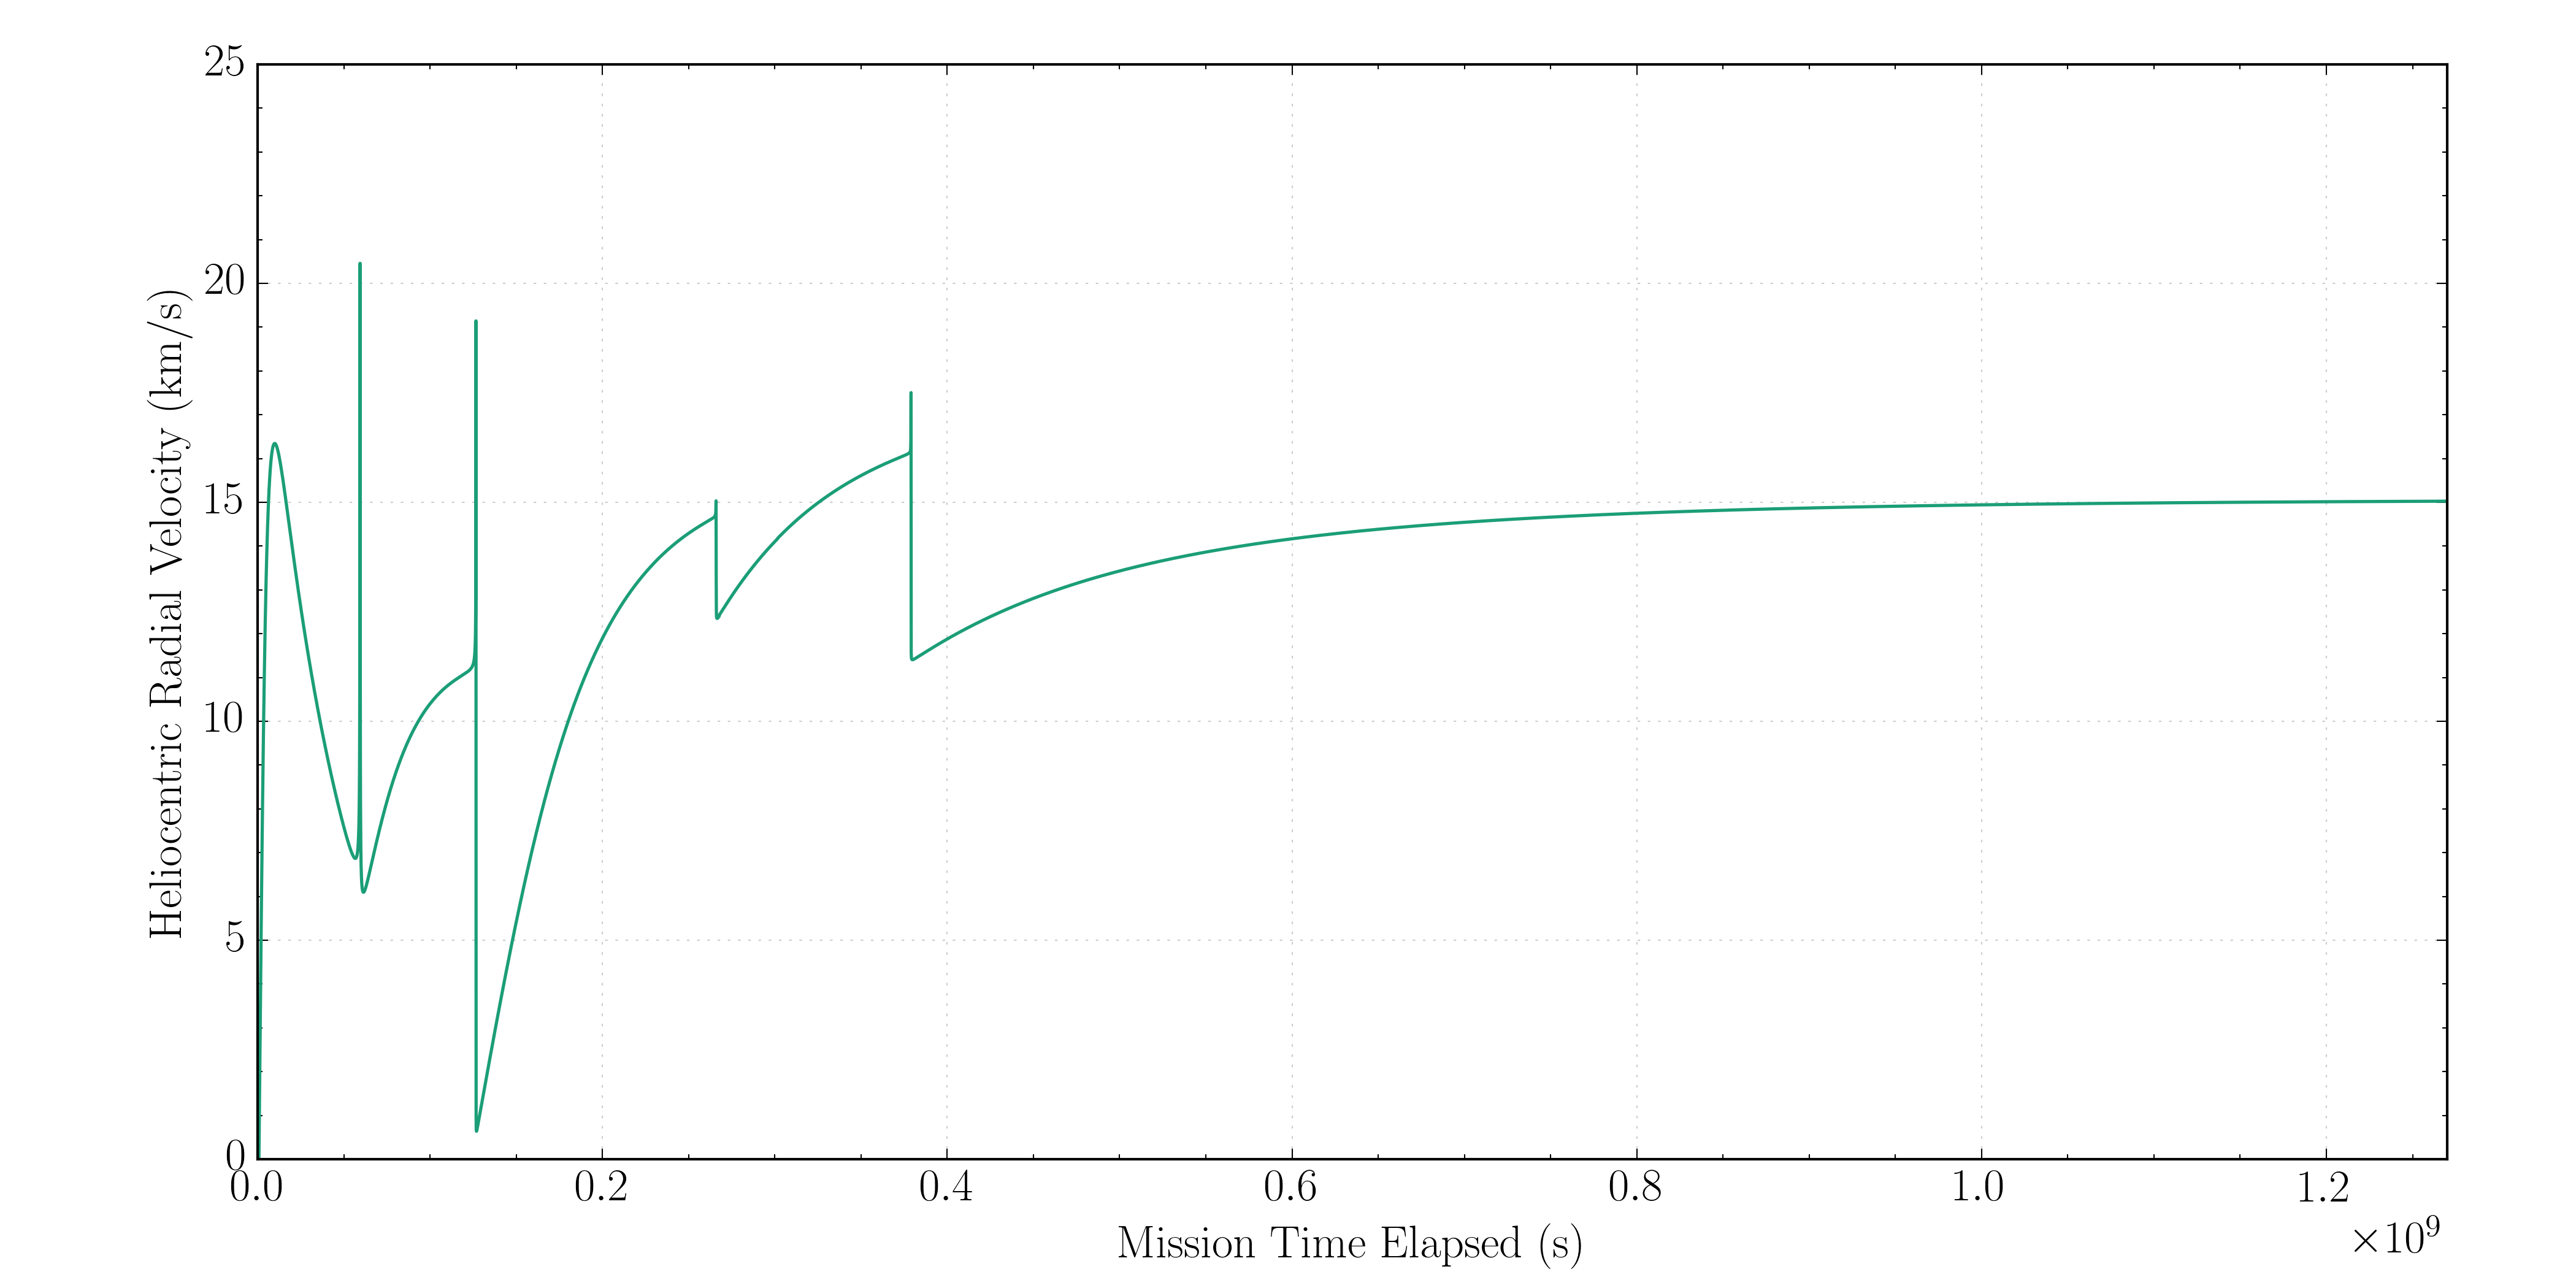
\includegraphics[width=\textwidth]{Voyager_Trajectory.png}
		\caption{Heliocentric radial velocity of the Voyager 2 probe.  Data courtesy of JPL-Horizons (ssd.jpl.nasa.gov/?horizons).}
	\end{figure}
	
\end{document}
